\documentclass[conference,onecolumn]{IEEEtran}
\usepackage{enumitem}
\usepackage{cite}
\usepackage{graphicx}
\usepackage{float}
\graphicspath{{./images}}

\title{XM Radio Reception with the PlutoSDR}

\author{
\IEEEauthorblockN{Owen Sowatzke}
\IEEEauthorblockA{\textit{Electrical Engineering Department} \\
\textit{University of Arizona}\\
Tucson, USA \\
osowatzke@arizona.edu}
\and
\IEEEauthorblockN{Glenn Alan Walker}
\IEEEauthorblockA{\textit{Electrical Engineering Department} \\
\textit{University of Arizona}\\
Tucson, USA \\
gaw@arizona.edu}}

\begin{document}
\maketitle

XM radio leverages a combination of satellites and terrestrial repeaters to diversify its transmitted signal. The satellites transmit QSPK-modulated symbols, and the terrestrial repeaters leverage COFDM modulation \cite{5586866}. For our final project, we propose demodulating the signal from a single satellite and performing forward error correction (FEC). Our project will leverage the time, frequency, and frame synchronization methods covered in class. Additionally, it will extend the material covered in class to forward error correction. XM radio is a proprietary signal, and the technical details are documented only in patents such as \cite{a2008_us8260192b2, marko_2012_us8667344b2}. Major milestones for our project include: performing timing and frequency synchronization, extracting the master frame preamble (MFP) and frame synchronization preamble (FSP), and demodulating the signal from a single satellite. Additional stretch goals that will be addressed only if time permits include: demodulating the COFDM signals from terrestrial repeaters, combining the returns from multiple satellites and/or the terrestrial repeaters, and playing XM channel 1 audio (free preview channel). We believe that this project will reinforce what we learned in the course and provide invaluable experience performing FEC and OFDM demodulation.

\iffalse
\begin{figure}[H]
	\centerline{\fbox{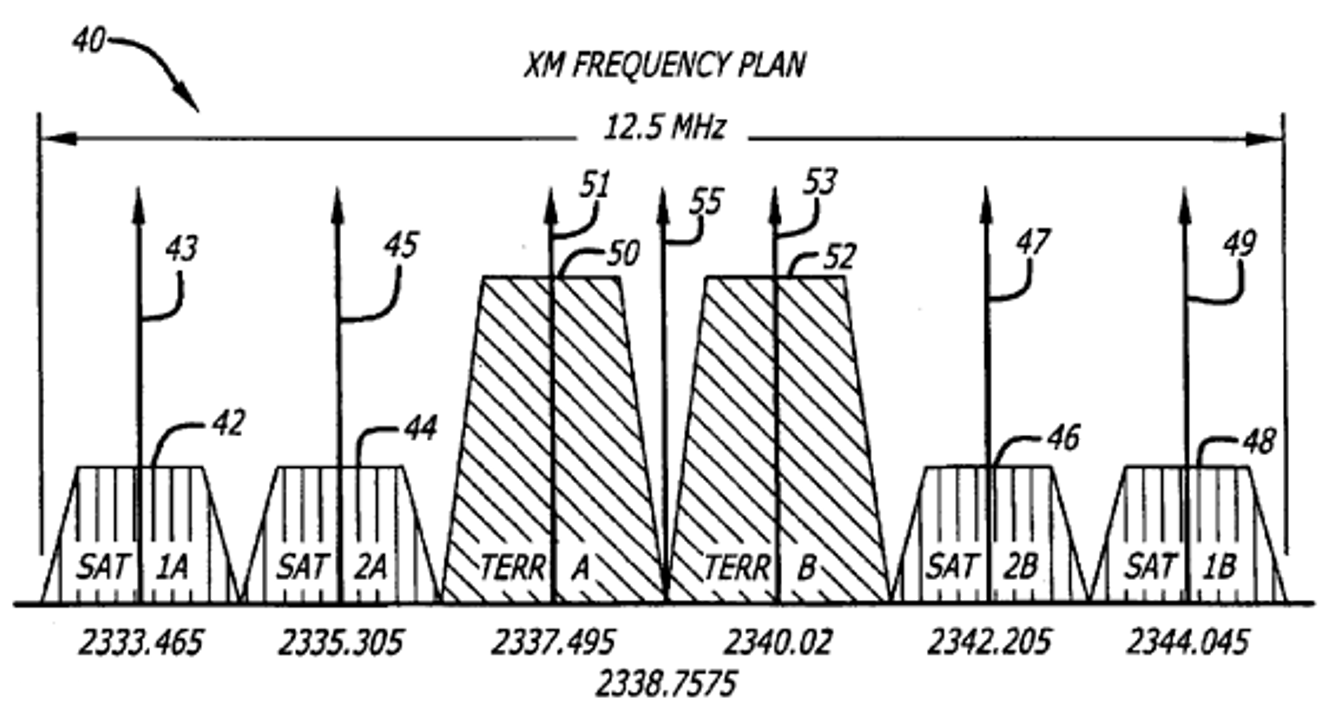
\includegraphics[width=0.5\textwidth]{xm_spectrum.png}}}
	\caption{XM Radio Spectrum \cite{a1999_us6724827b1}}
	\label{fig::xm_spectrum}
\end{figure}
\fi

\begin{figure}[H]
	\centerline{\fbox{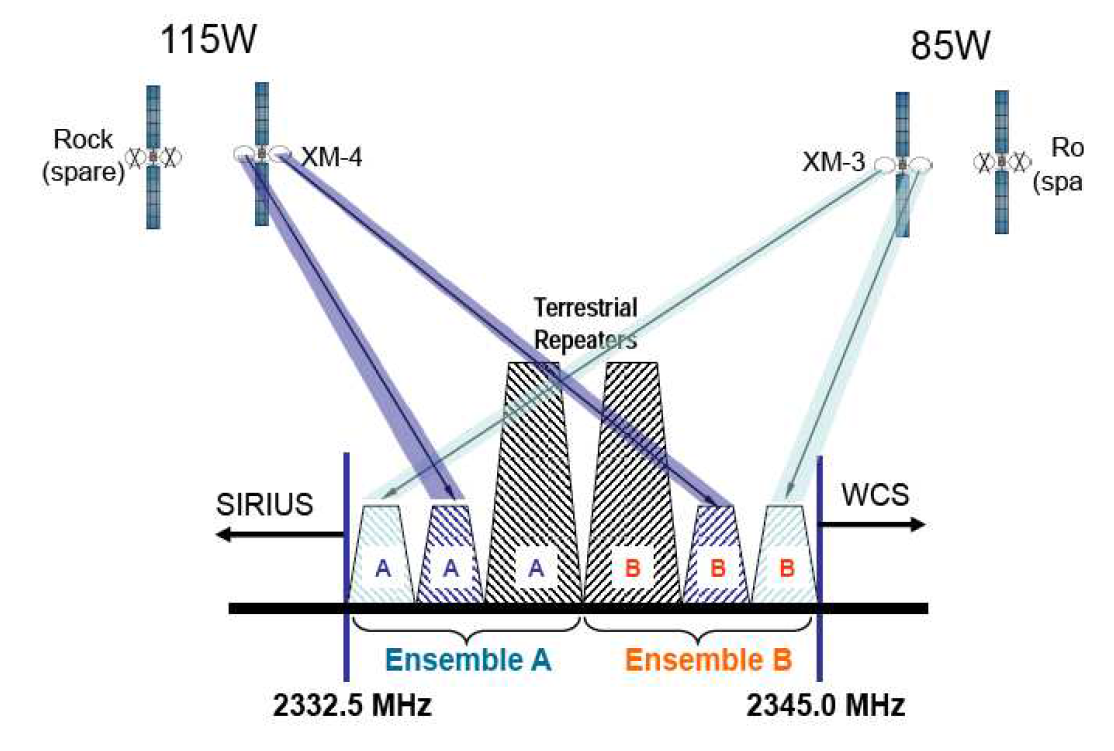
\includegraphics[width=0.5\textwidth]{xm_satellite_config.png}}}
	\caption{XM Radio Satellite Configuration \cite{5586866}}
	\label{fig::xm_satellite_config}
\end{figure}

XM Radio divides their content across two separate ensembles (Ensemble A and Ensemble B), which are illustrated in Figure \ref{fig::xm_satellite_config}. Each ensemble uses transmitter diversity to improve signal quality and prevent dropouts. The diversity scheme specifically uses QPSK-modulated signals from two separate satellites and a terrestrial COFDM-modulated signal. We concentrate specifically on the TDM receiver. An example of its architecture is displayed in Figure \ref{fig::tdm_receiver}. 

\begin{figure}[H]
	\centerline{\fbox{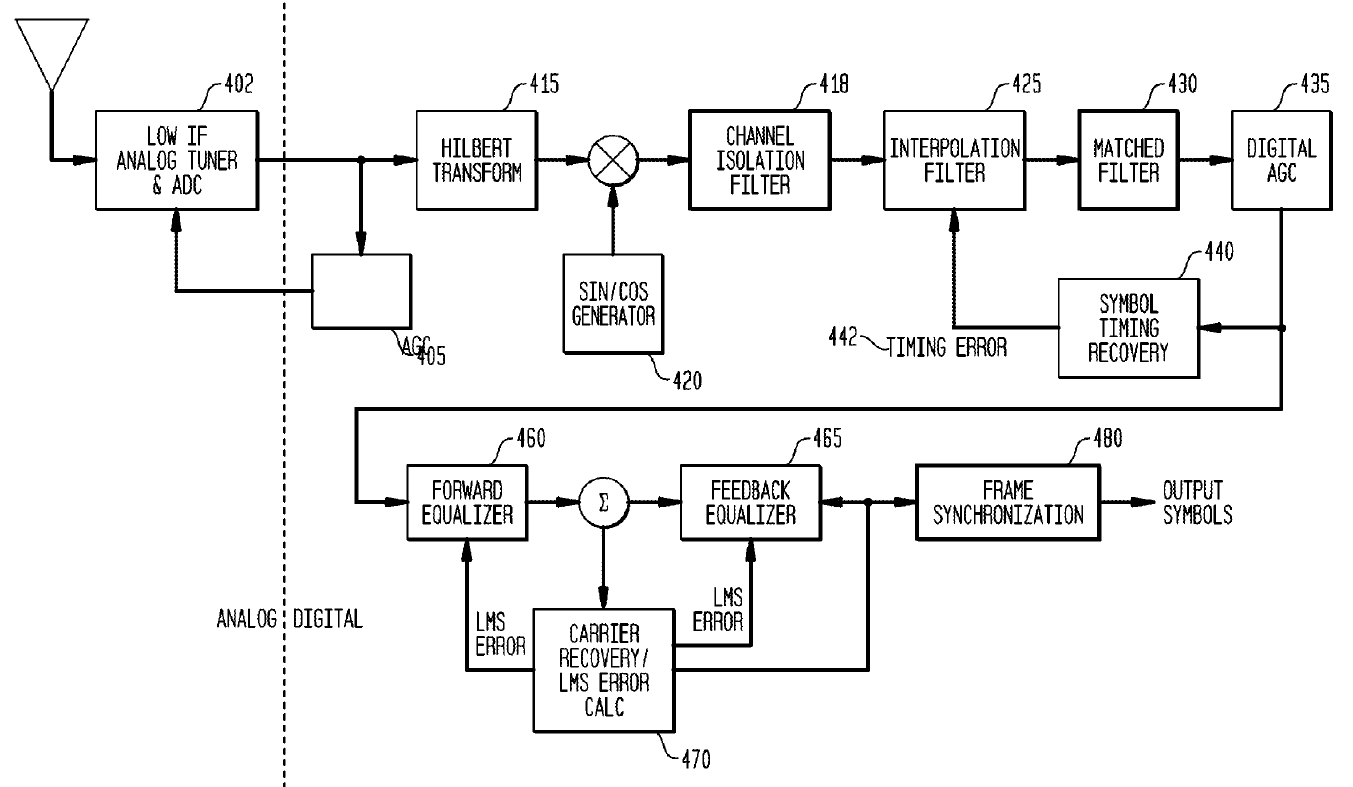
\includegraphics[width=0.5\textwidth]{tdm_receiver.png}}}
	\caption{TDM Receiver Architecture \cite{a2008_us8260192b2}}
	\label{fig::tdm_receiver}
\end{figure}

\begin{figure}[H]
	\centerline{\fbox{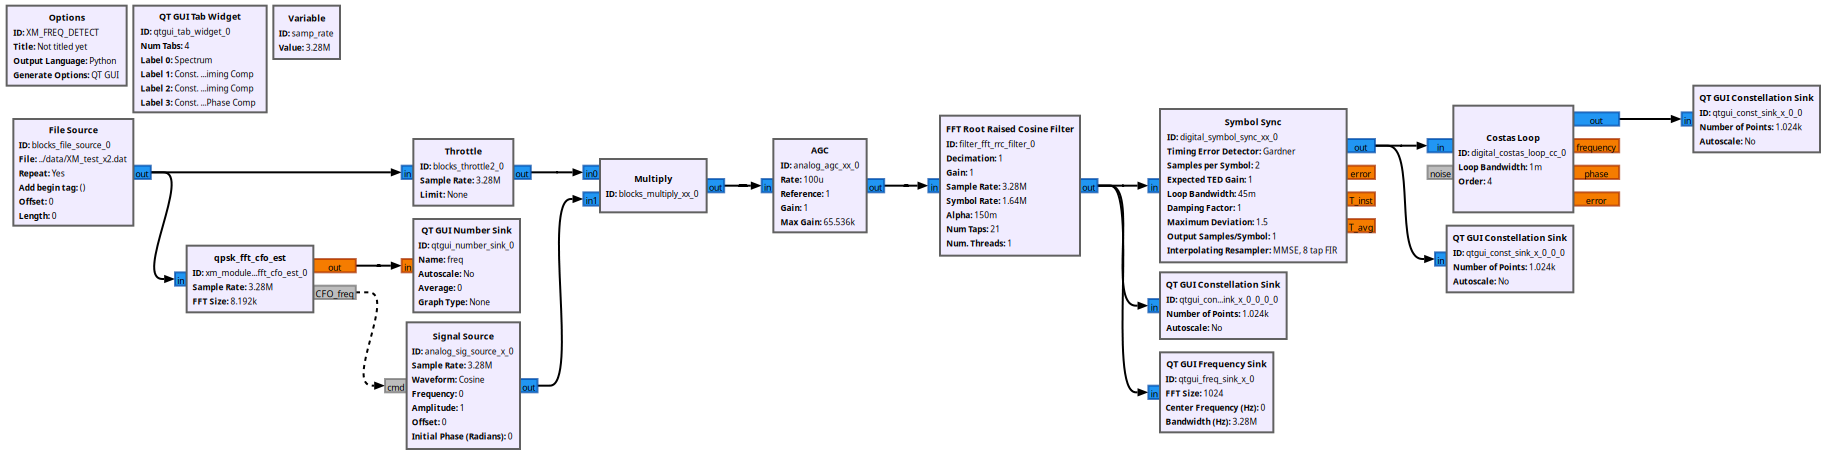
\includegraphics[width=0.8\textwidth]{timing_carrier_sync.png}}}
	\caption{GNU Radio Flowchart That Implements Timing and Carrier Synchronization}
	\label{fig::timing_carrier_sync}
\end{figure}

The XM radio signal is transmitted through a square-root raised cosine filter, which limit the signal bandwidth [ADD A CITATION HERE]. Because of this, the receiver needs a matching square root raised cosine filter. The root-raised cosine filter is a type II Nyquist filter, which results in zero intersymbol interference when the received signal is sampled at the midpoint of each symbol period. When the PlutoSDR samples the received signal, this condition is not strictly enforced. This results in significant spreading in our constellation as illustrated in Figure \ref{fig::constellation_no_timing_comp}.

\begin{figure}[H]
	\centerline{\fbox{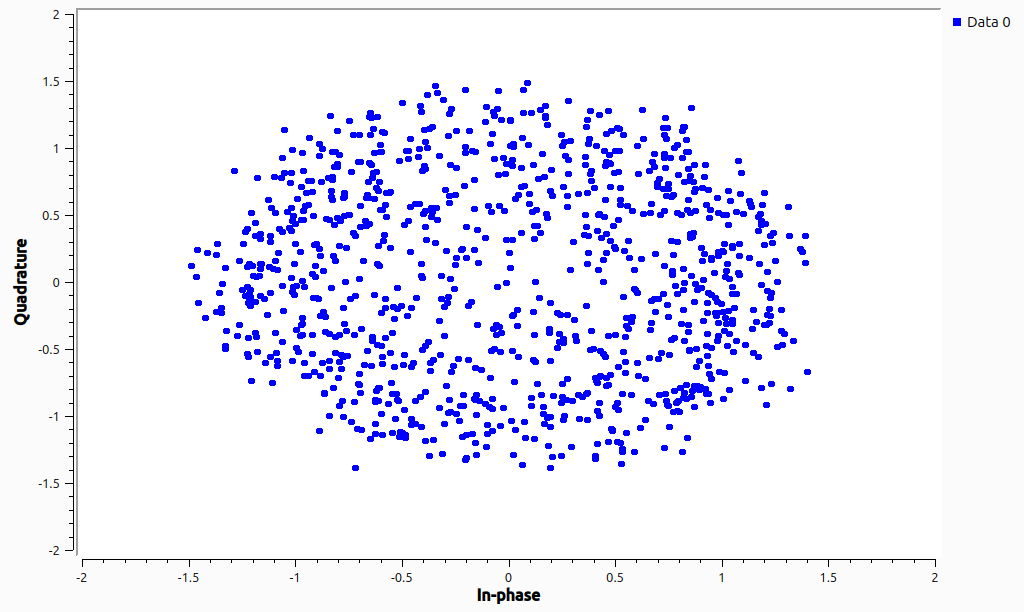
\includegraphics[width=0.5\textwidth]{constellation_no_timing_comp.png}}}
	\caption{Received Constellation Before Timing Synchronization}
	\label{fig::constellation_no_timing_comp}
\end{figure}

We can correct for this timing offset using a timing synchronization block. For this purpose, we use a GNU radio symbol sync block. This symbol sync block can be subdivided into 4 blocks: interpolator, timing error detector, loop filter, and controller. The interpolator applies a fractional delay. The timing error detector measures the timing offset. The loop filter stabilizes the process. And the controller manages the interpolation process. For our work, we specifically choose a Gardner Timing Error detector because it is robust to frequency errors. Our constellation after timing compensation is shown in Figure \ref{fig::constellation_after_timing_comp}.

\begin{figure}[H]
	\centerline{\fbox{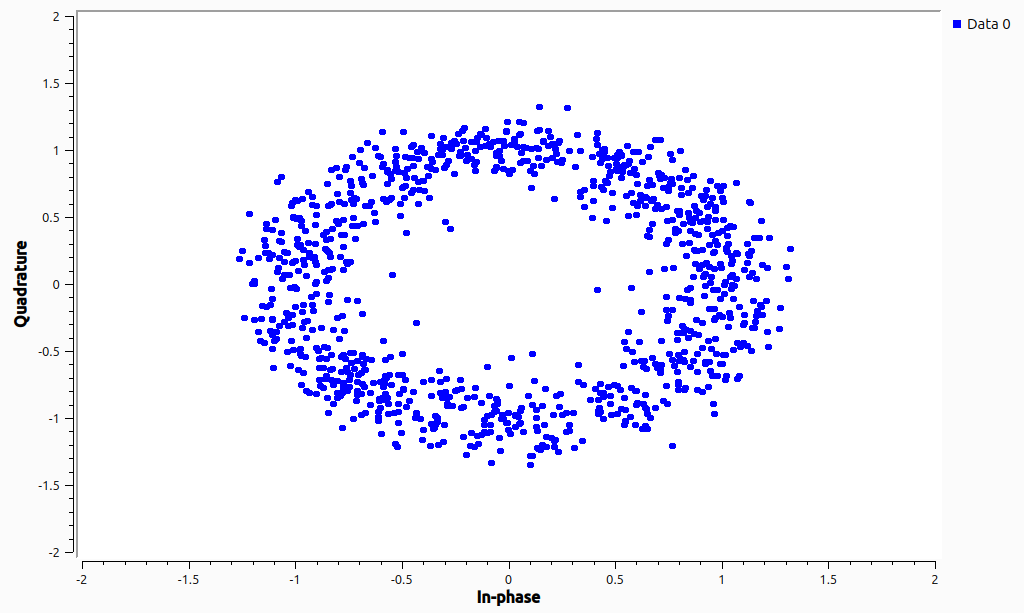
\includegraphics[width=0.5\textwidth]{constellation_after_timing_comp.png}}}
	\caption{Received Constellation After Timing Synchronization}
	\label{fig::constellation_after_timing_comp}
\end{figure}

After timing compensation, we see that the amplitude of the constellation has stabilized. However, the resulting constellation is a ring. This occurs because after phase and frequency errors. The phase error leads to a static tilt of the constellation and the frequency offset causes our constellation to rotate. To correctly demodulate the signal, we must also remove the frequency offset in the signal. We do this in 2 stages: coarse frequency compensation and fine frequency compensation. We implement the coarse frequency compensation algorithm using a custom GNU radio python block. This block raises our received data to the fourth power to remove the QPSK modulation. Then, it takes an FFT of the resulting signal. The peak index of the FFT provides us with an estimate of the coarse frequency error. When solving for the error we also must divide the frequency error by 4 to account for raising the received data to the 4th power prior to the FFT. The FFT output and the corresponding frequency error for one frame of data is shown in Figure \ref{fig::cfo_frequency_estimate}. Examining the Figure, we observe a frequency error of roughly 15 kHz [CHECK SIGN].

\begin{figure}[H]
	\centerline{\fbox{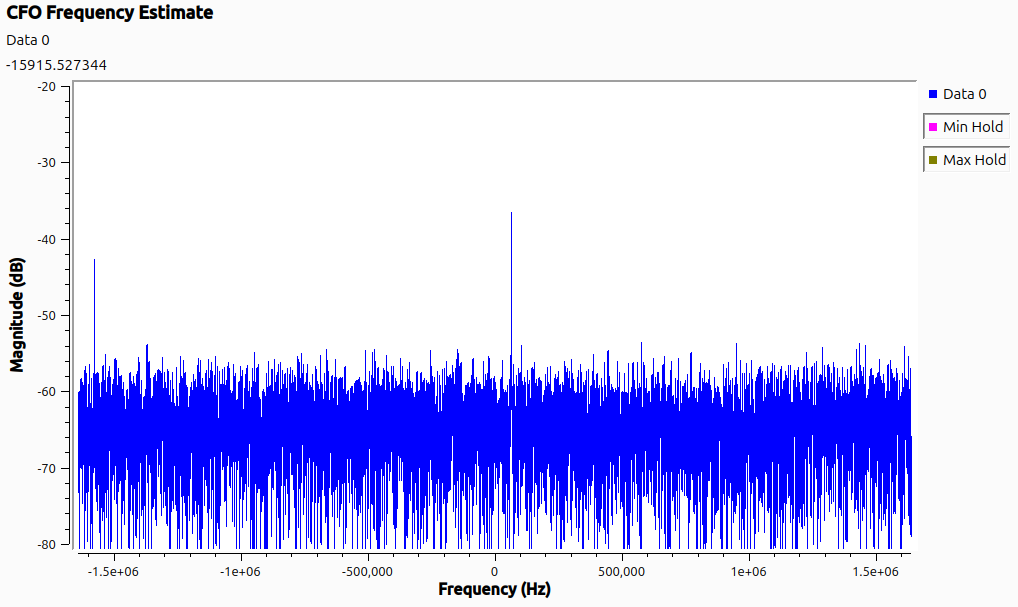
\includegraphics[width=0.5\textwidth]{cfo_frequency_estimate.png}}}
	\caption{Coarse Frequency FFT Output}
	\label{fig::cfo_frequency_estimate}
\end{figure}

The coarse frequency compensation is limited by the FFT size and the rate at which the frequency drifts. We add an additional fine frequency compensation block to resolve the rest of the error. We use the GNU radio Costas Loop block for this analysis. The GNU radio Costas Loop closely resembles the timing synchronization block. It includes a phase error detector, a loop filter, a direct digital synthesizer and a phase rotator.
The phase rotator adjusts the phase of the received signal by multiplying it with a phasor. The phase error detector then detects the phase error, which is fed into a loop filter for stabilization. Finally the Direct Digital Synthesizer creates a coherent phasor which removes residual phase and frequency offsets. The constellation after fine frequency compensation is shown in Figure \ref{fig::constellation_after_fine_carrier_comp}.

\begin{figure}[H]
	\centerline{\fbox{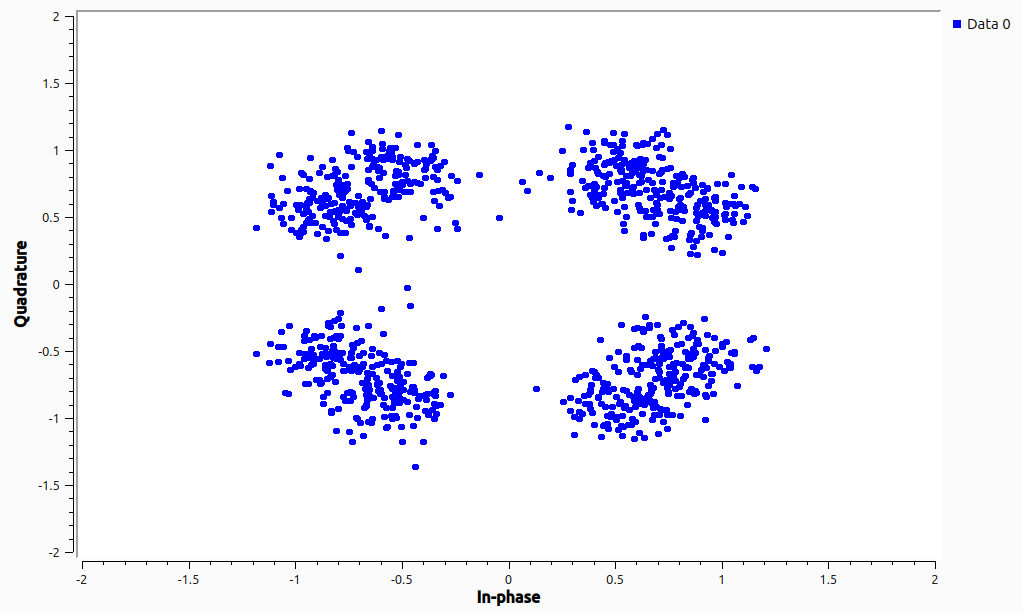
\includegraphics[width=0.5\textwidth]{constellation_after_fine_carrier_comp.png}}}
	\caption{Received Constellation After Fine Carrier Synchronization}
	\label{fig::constellation_after_fine_carrier_comp}
\end{figure}

XM radio divides its transmitted data into frames. These frames are marked by two different preambles: the MFP (master frame preamble) and the FSP (fast synchronization preamble). The FSP marks the start of the data portion and corrects for ambiguities, while the MFP is used to align the signal from each satellite \cite{a2008_us8260192b2}. Both preambles and their relative timing are illustrated in Figure \ref{fig::tdm_frame_format}.

\begin{figure}[H]
	\centerline{\fbox{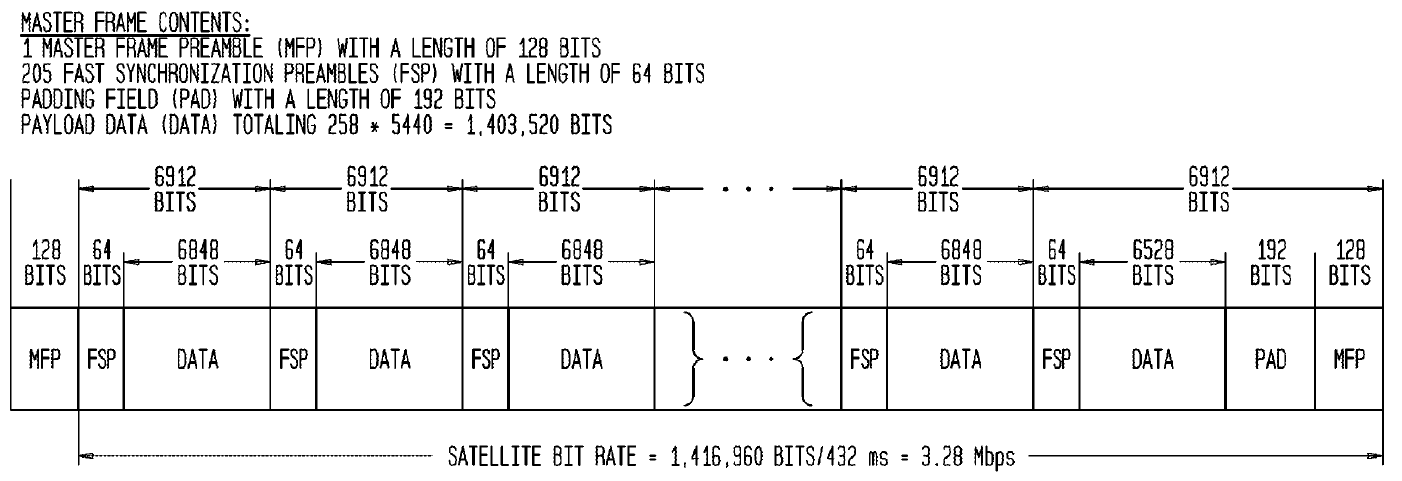
\includegraphics[width=0.8\textwidth]{tdm_frame_format.png}}}
	\caption{TDM Frame Format \cite{a2008_us8260192b2}}
	\label{fig::tdm_frame_format}
\end{figure}

The patents we referenced did not provide the MFP or FSP. As a result, we identified them ourselves using the auto-correlation of our signal. We considered the FSP first because it occurred more frequently in our collected data. To compute the FSP, we correlated an FSP duration of samples with a copy delayed by the FSP separation. By sweeping the starting index until we maximized the auto-correlation, we were able to effectively identify the start of our FSP. Our approach is illustrated in Figure \ref{fig::finding_fsp} and the best auto-correlation is shown in Figure \ref{fig::fsp_correlation}.

\begin{figure}[H]
	\centerline{\fbox{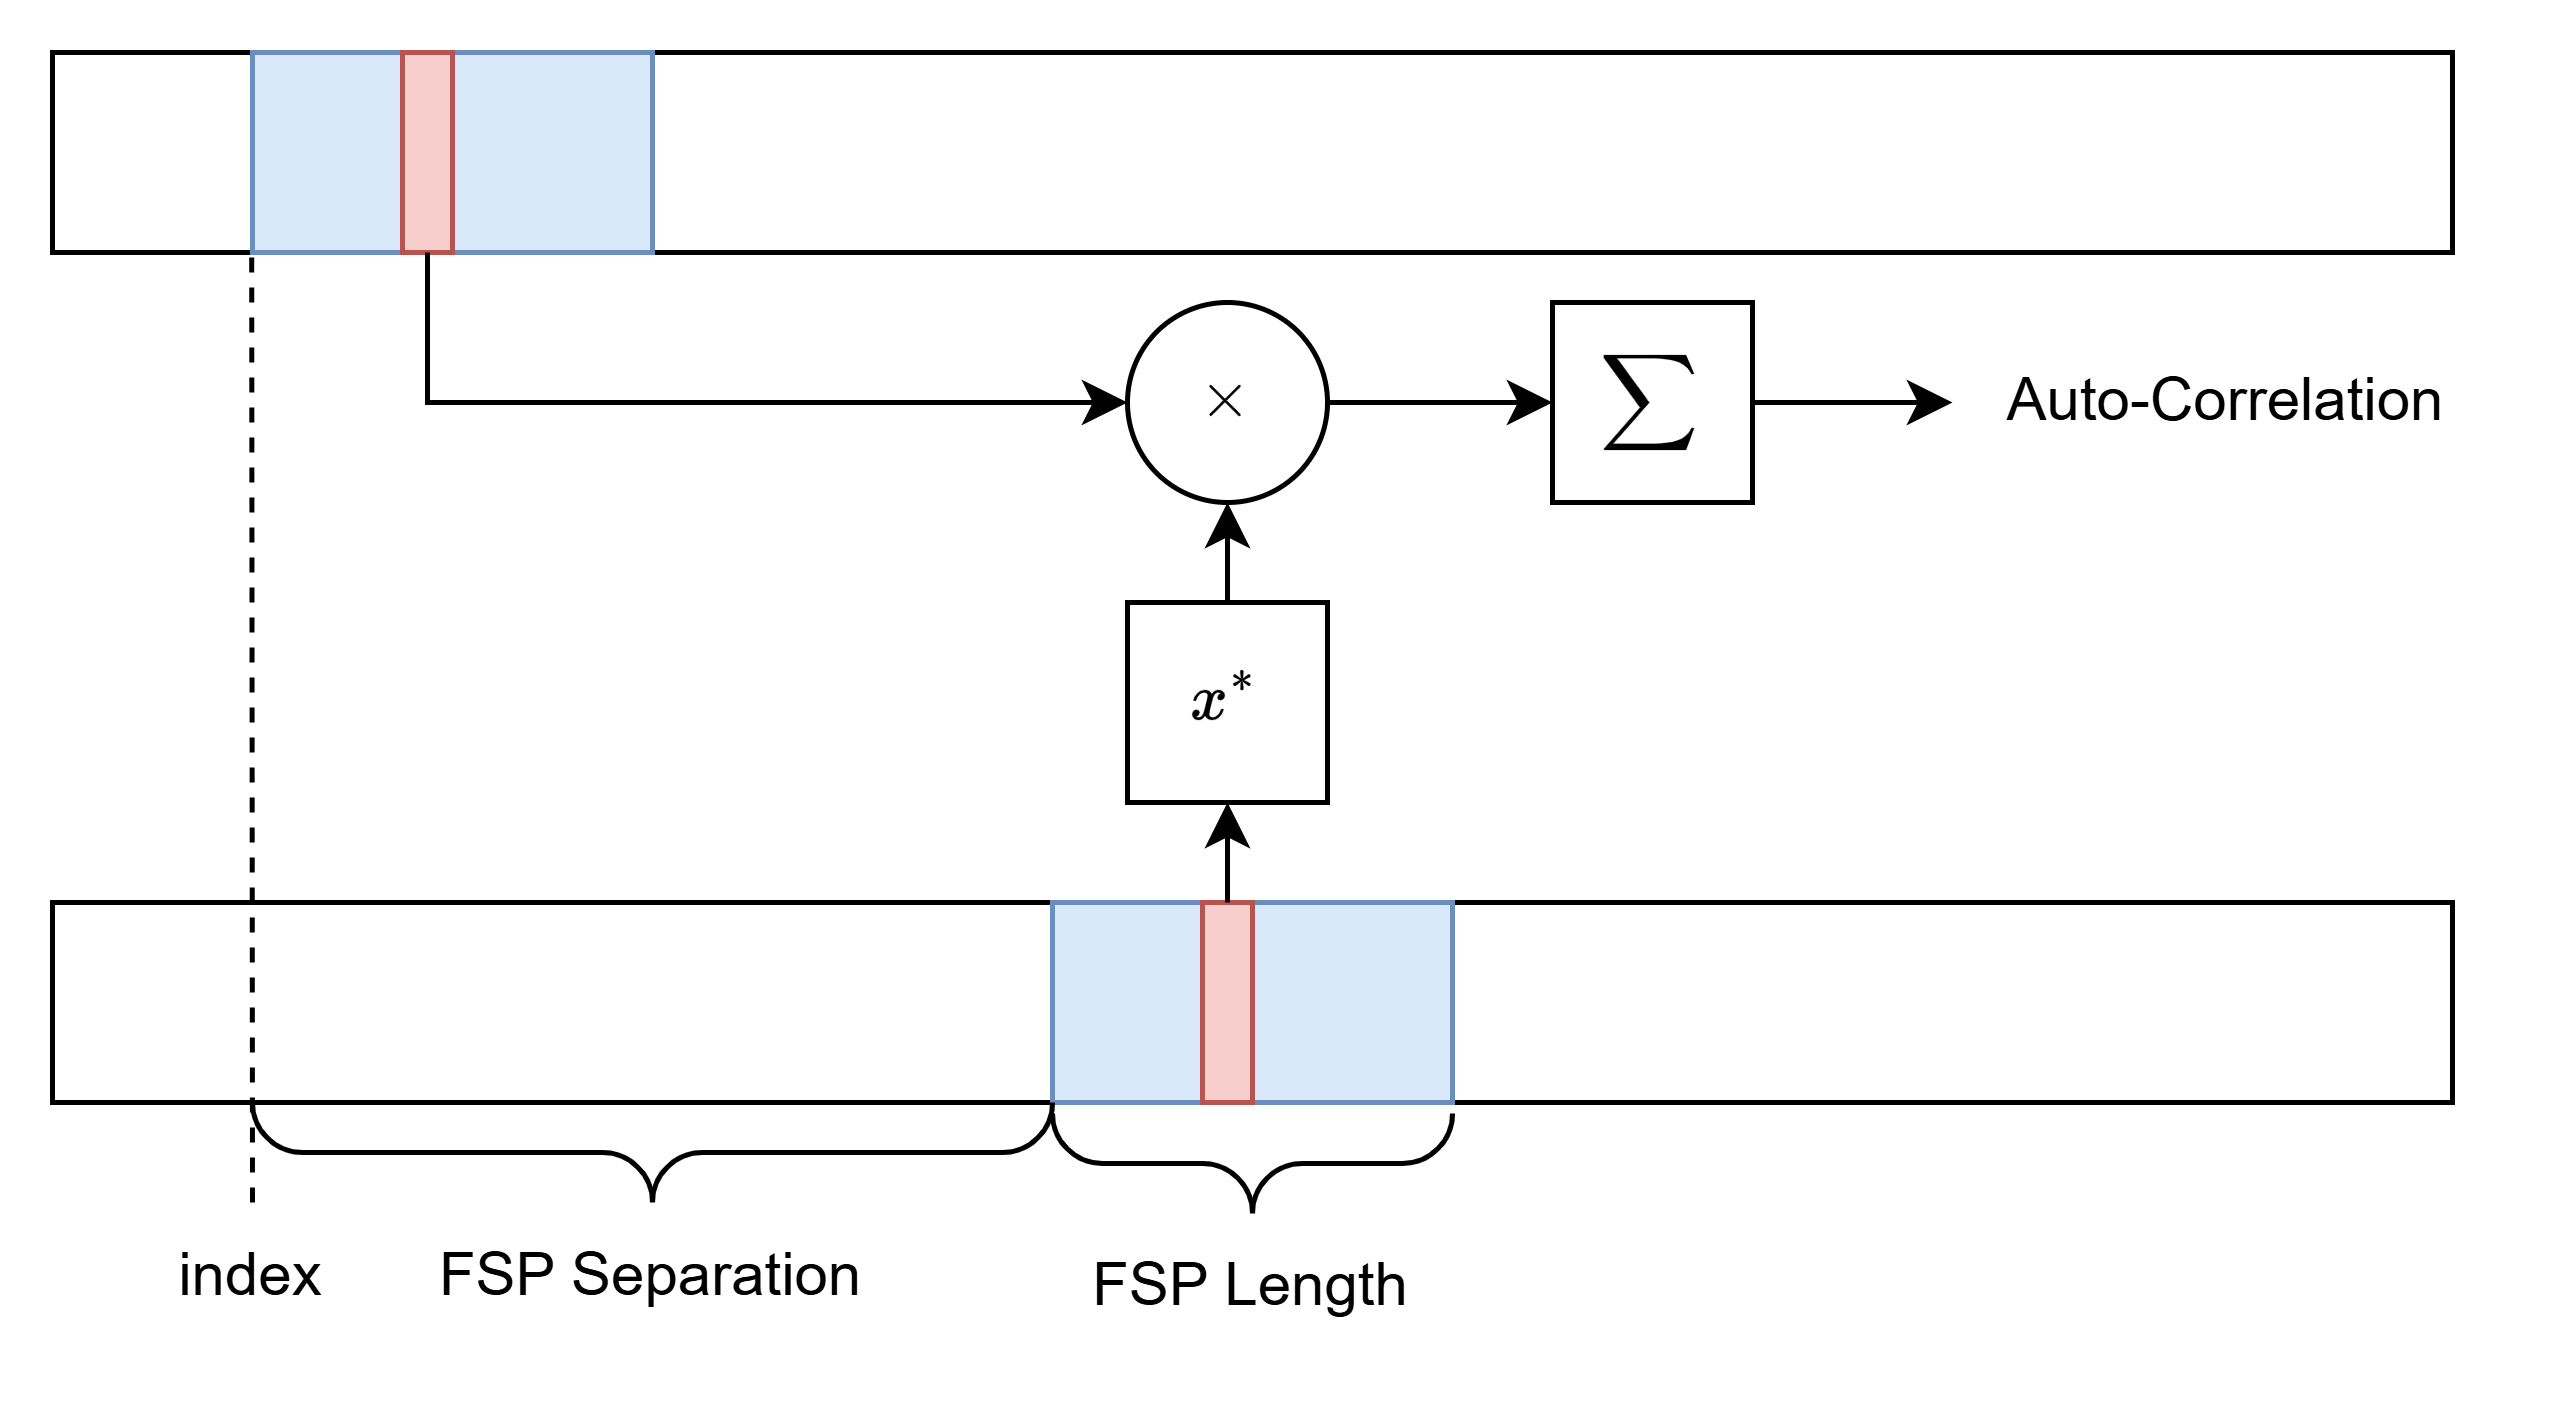
\includegraphics[width=0.5\textwidth]{finding_fsp.png}}}
	\caption{Algorithm for Indentifying FSP}
	\label{fig::finding_fsp}
\end{figure}

\begin{figure}[H]
	\centerline{\fbox{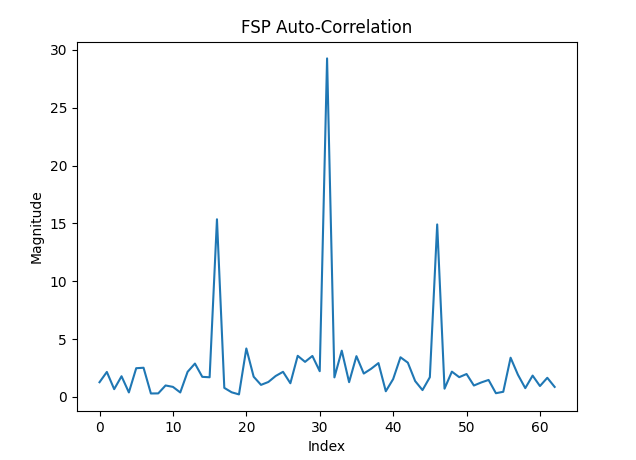
\includegraphics[width=0.5\textwidth]{fsp_correlation.png}}}
	\caption{Auto-Correlation of Optimum FSP Selection}
	\label{fig::fsp_correlation}
\end{figure}

cross-correlated the signal with delayed versions of itself. When the cross-correlation output peaked, we selected the preamble-length set of samples that resulted in a peak as the preamble. We also demodulated the signal using BPSK demodulation to reconstruct the original preamble. The maximum cross-correlation output when identifying the master frame preamble is shown in Figure \ref{fig::mfp_correlation}.\\


\begin{figure}[H]
	\centerline{\fbox{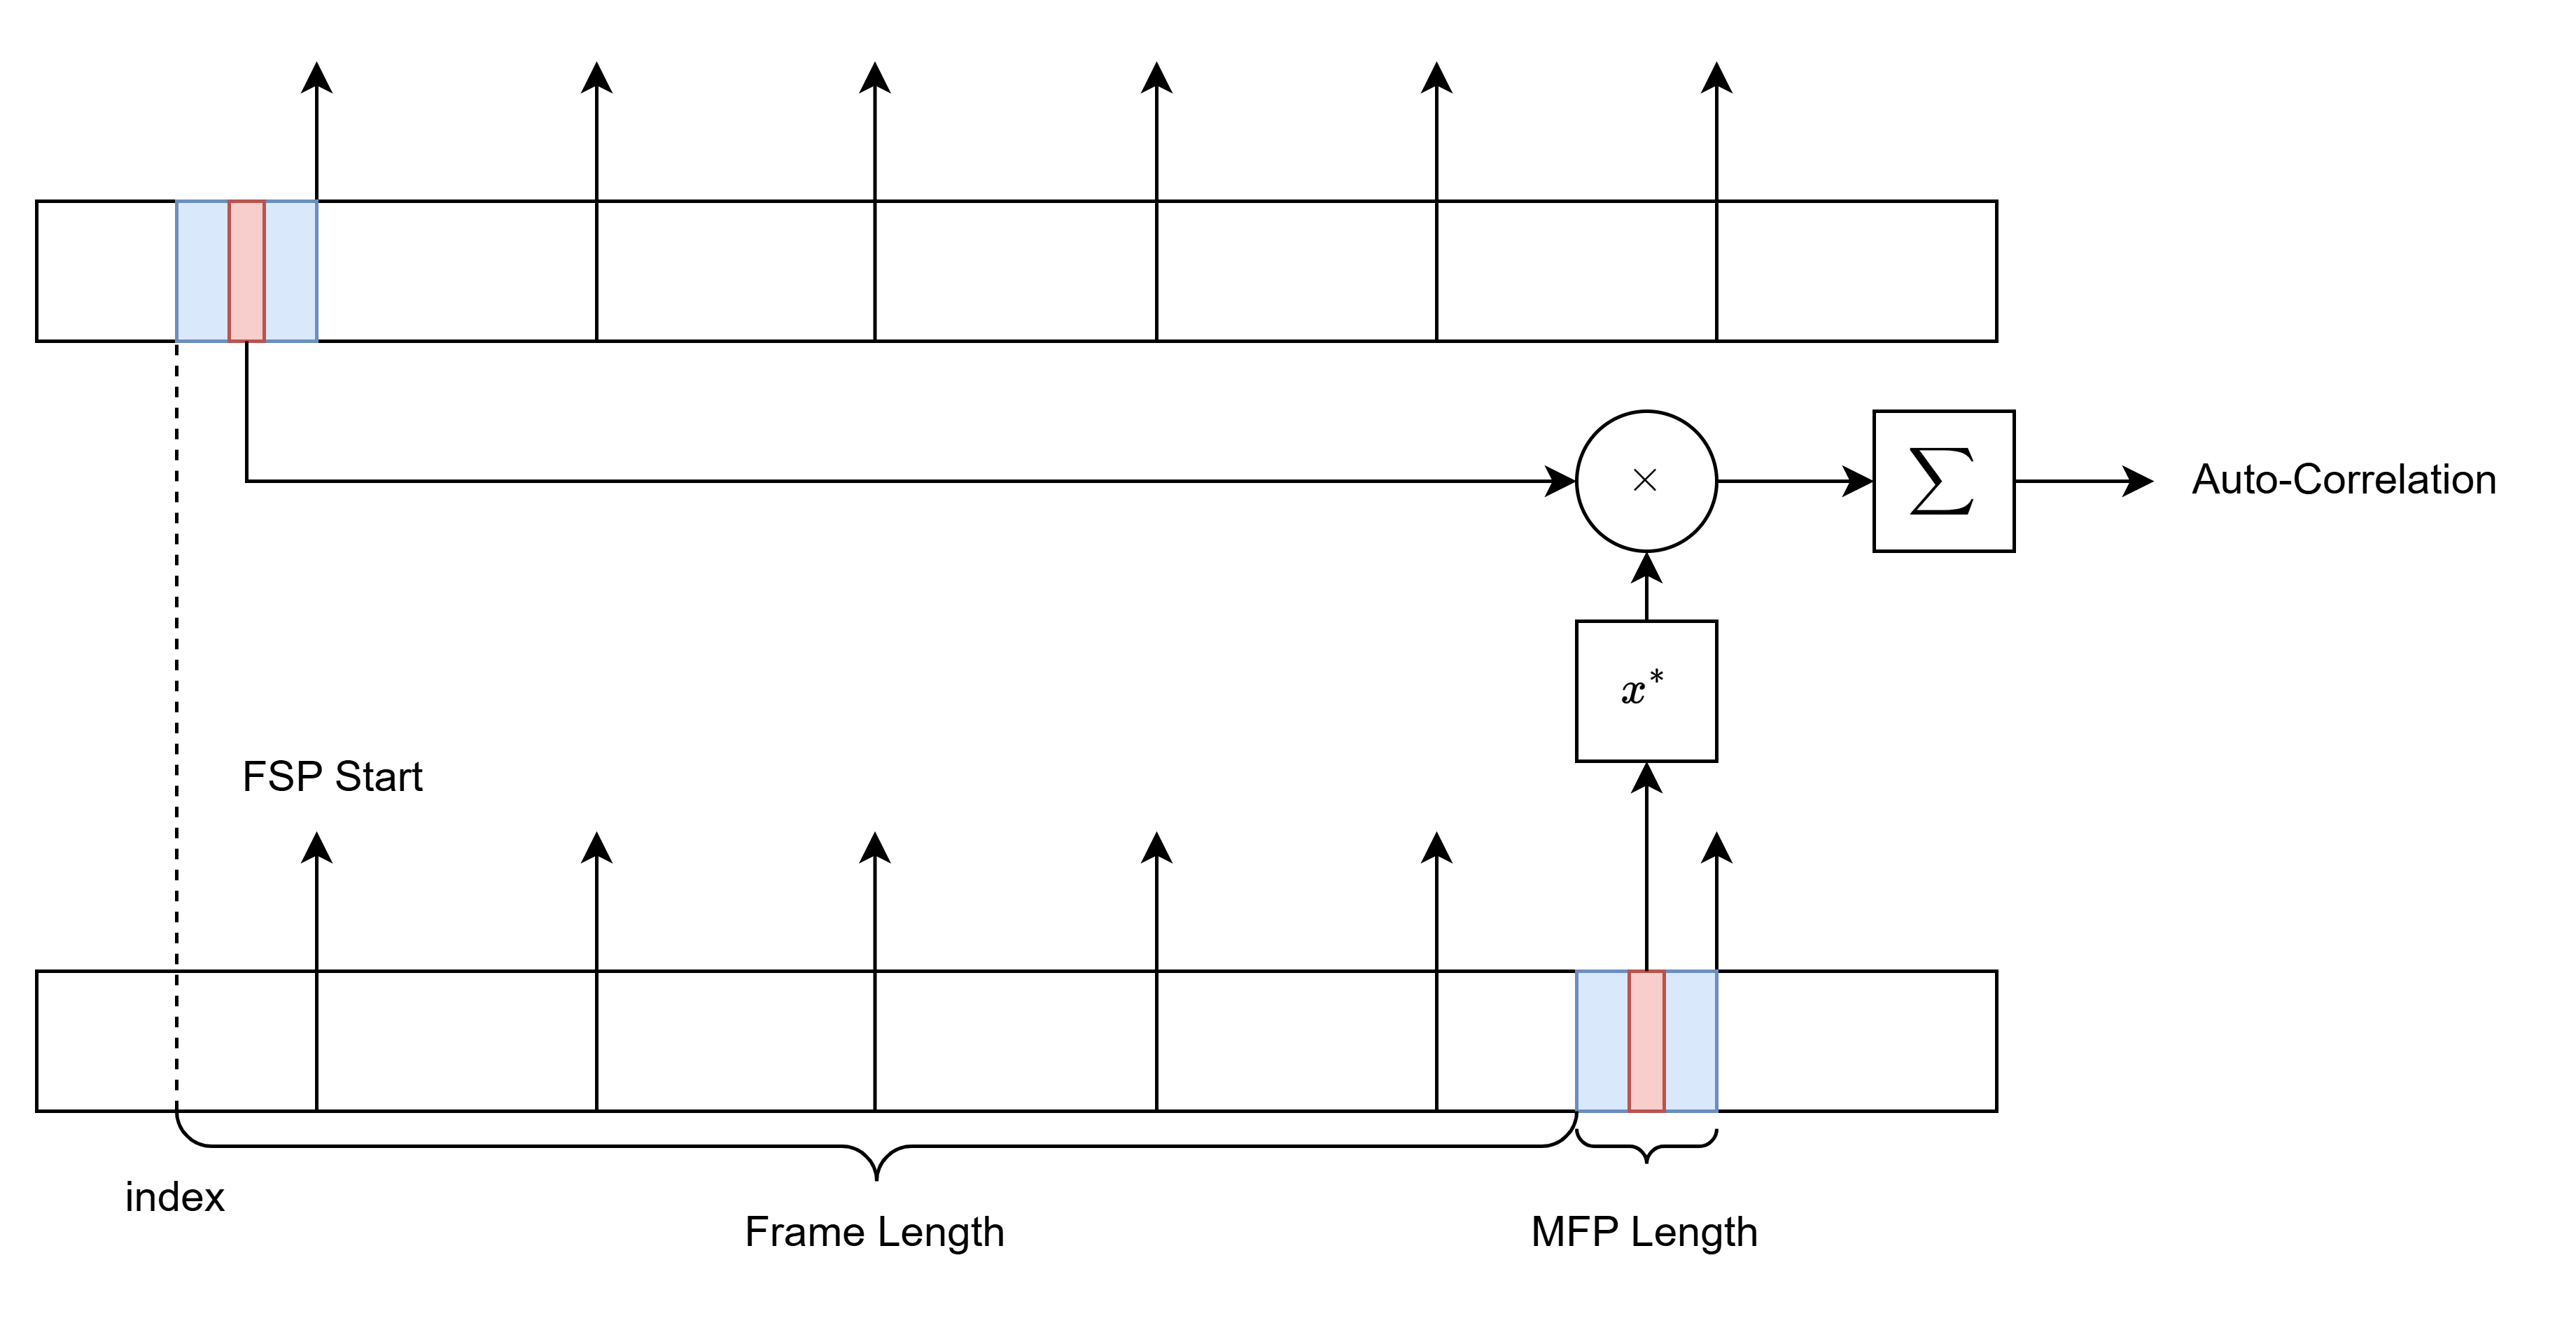
\includegraphics[width=0.5\textwidth]{finding_mfp.png}}}
	\caption{Algorithm for Indentifying MFP}
	\label{fig::finding_mfp}
\end{figure}



\begin{figure}[H]
	\centerline{\fbox{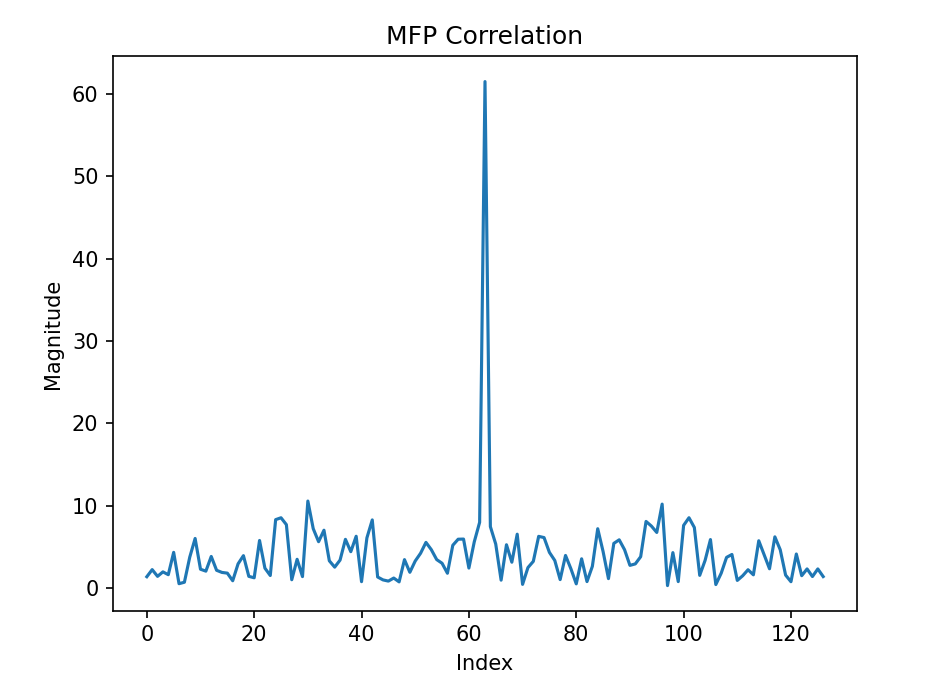
\includegraphics[width=0.5\textwidth]{mfp_correlation.png}}}
	\caption{Finding the MFP using Cross Correlation}
	\label{fig::mfp_correlation}
\end{figure}

% Add plot of FSP in constellation w/ different color

% Add picture of setup

\begin{itemize}
	\item Nyquist Filter
	\item Timing Synchronization
	\item Carrier Compensation
	\begin{itemize}
		\item Coarse
		\item Fine
	\end{itemize}
	\item Frame Synchronization
\end{itemize}

\nocite{5586866}
\nocite{a2008_us8260192b2}
\nocite{marko_2012_us8667344b2}
\nocite{collins_2018_softwaredefined}
\nocite{chaudhari_2022_timing}
\nocite{650240}
\bibliographystyle{IEEEtran}
\bibliography{sources}{}
%\bibliographystyle{ieeetr}
\end{document}